\documentclass[xcolor={dvipsnames}]{beamer}
%\usepackage[utf8]{inputenc}
%\usetheme{Madrid}
\usetheme{CambridgeUS}
%\usetheme{Malmoe}
%\usecolortheme{beaver}
\usecolortheme{seahorse}

%-------------------------------------------------------------------------------
%          -Packages nécessaires pour écrire en Français et en UTF8-
%-------------------------------------------------------------------------------
\usepackage[utf8]{inputenc}
\usepackage[frenchb]{babel}
\usepackage[T1]{fontenc}
\usepackage{lmodern}
\usepackage{textcomp}

%-------------------------------------------------------------------------------

%-------------------------------------------------------------------------------
%                          -Outils de mise en forme-
%-------------------------------------------------------------------------------
\usepackage{hyperref}
\hypersetup{pdfstartview=XYZ}
\usepackage{enumerate}
\usepackage{graphicx}
%\usepackage{multicol}
%\usepackage{tabularx}

%\usepackage{anysize} %%pour pouvoir mettre les marges qu'on veut
%\marginsize{2.5cm}{2.5cm}{2.5cm}{2.5cm}

\usepackage{indentfirst} %%pour que les premier paragraphes soient aussi indentés
\usepackage{verbatim}
%\usepackage[table]{xcolor}  
%\usepackage{multirow}
\usepackage{ulem}
%-------------------------------------------------------------------------------


%-------------------------------------------------------------------------------
%                  -Nécessaires pour écrire des mathématiques-
%-------------------------------------------------------------------------------
\usepackage{amsfonts}
\usepackage{amssymb}
\usepackage{amsmath}
\usepackage{amsthm}
\usepackage{tikz}
\usepackage{xlop}
\usepackage[output-decimal-marker={,}]{siunitx}
%-------------------------------------------------------------------------------


%-------------------------------------------------------------------------------
%                    - Mise en forme 
%-------------------------------------------------------------------------------

\newcommand{\bu}[1]{\underline{\textbf{#1}}}


\usepackage{ifthen}


\newcommand{\ifTrue}[2]{\ifthenelse{\equal{#1}{true}}{#2}{$\qquad \qquad$}}

\newcommand{\kword}[1]{\textcolor{red}{\underline{#1}}}


%-------------------------------------------------------------------------------



%-------------------------------------------------------------------------------
%                    - Racourcis d'écriture -
%-------------------------------------------------------------------------------

% Angles orientés (couples de vecteurs)
\newcommand{\aopp}[2]{(\vec{#1}, \vec{#2})} %Les deuc vecteurs sont positifs
\newcommand{\aopn}[2]{(\vec{#1}, -\vec{#2})} %Le second vecteur est négatif
\newcommand{\aonp}[2]{(-\vec{#1}, \vec{#2})} %Le premier vecteur est négatif
\newcommand{\aonn}[2]{(-\vec{#1}, -\vec{#2})} %Les deux vecteurs sont négatifs

%Ensembles mathématiques
\newcommand{\naturels}{\mathbb{N}} %Nombres naturels
\newcommand{\relatifs}{\mathbb{Z}} %Nombres relatifs
\newcommand{\rationnels}{\mathbb{Q}} %Nombres rationnels
\newcommand{\reels}{\mathbb{R}} %Nombres réels
\newcommand{\complexes}{\mathbb{C}} %Nombres complexes


%Intégration des parenthèses aux cosinus
\newcommand{\cosP}[1]{\cos\left(#1\right)}
\newcommand{\sinP}[1]{\sin\left(#1\right)}

%Fractions
\newcommand{\myfrac}[2]{{\LARGE $\frac{#1}{#2}$}}

%Vocabulaire courrant
\newcommand{\cad}{c'est-à-dire}

%Droites
\newcommand{\dte}[1]{droite $(#1)$}
\newcommand{\fig}[1]{figure $#1$}
\newcommand{\sym}{symétrique}
\newcommand{\syms}{symétriques}
\newcommand{\asym}{axe de symétrie}
\newcommand{\asyms}{axes de symétrie}
\newcommand{\seg}[1]{$[#1]$}
\newcommand{\monAngle}[1]{$\widehat{#1}$}
\newcommand{\bissec}{bissectrice}
\newcommand{\mediat}{médiatrice}
\newcommand{\ddte}[1]{$[#1)$}

%Figures
\newcommand{\para}{parallélogramme}
\newcommand{\paras}{parallélogrammes}
\newcommand{\myquad}{quadrilatère}
\newcommand{\myquads}{quadrilatères}
\newcommand{\co}{côtés opposés}
\newcommand{\diag}{diagonale}
\newcommand{\diags}{diagonales}
\newcommand{\supp}{supplémentaires}
\newcommand{\car}{carré}
\newcommand{\cars}{carrés}
\newcommand{\rect}{rectangle}
\newcommand{\rects}{rectangles}
\newcommand{\los}{losange}
\newcommand{\loss}{losanges}


%----------------------------------------------------


\usepackage{../../../../pas-math}
\usepackage{../../../../moncours_beamer}

\usepackage{amssymb,amsmath}


\newcommand{\myitem}{\item[\textbullet]}

\graphicspath{{../img/}}

\title{Séquence 6 : Symétrie axiale}
%\subtitle{Correction des exercices semaine du 18/05}
%\author{O. FINOT}\institute{Collège S$^t$ Bernard}

%
%\AtBeginSection[]
%{
%	\begin{frame}
%		\frametitle{}
%		\tableofcontents[currentsection, hideallsubsections]
%	\end{frame} 
%
%}
%
%
%\AtBeginSubsection[]
%{
%	\begin{frame}
%		\frametitle{Sommaire}
%		\tableofcontents[currentsection, currentsubsection]
%	\end{frame} 
%}

\begin{document}



\begin{frame}
  \titlepage 
\end{frame}

\section{Symétrique d'une figure par rapport à une droite}
	

\section{Médiatrice}

\begin{frame}
	\begin{mydef}
		
		\begin{itemize}
			\item La \kword{médiatrice} d'un segment est son axe de symétrie. \pause
			\item C'est la droite \kword{perpendiculaire à ce segment} qui \kword{passe par son milieu}.\pause 
		\end{itemize}
		
	\end{mydef}


\begin{myex}
	

	La droite $(d)$ est la médiatrice du segment $[AB]$.

	\begin{center}
		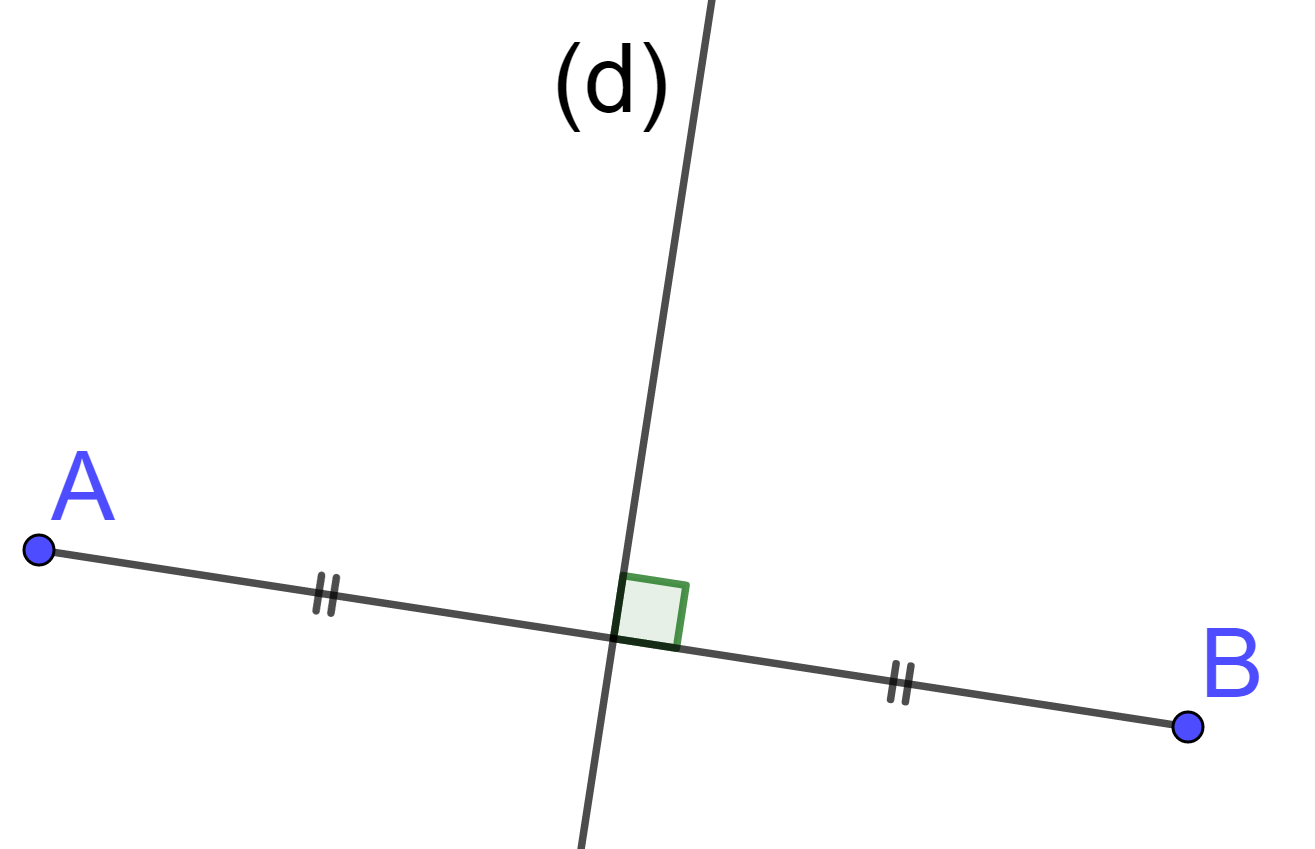
\includegraphics[scale=0.15]{med1}
	\end{center}
\end{myex}

\end{frame}

\begin{frame}
	\begin{myprops}
		\begin{itemize}
				\item \textbf{Si} un point appartient à la médiatrice d'un segment, \textbf{alors} ce point est à la même distance des extrémités de ce segment. \pause
				\item \textbf{Si} un point est à la même distance des extrémités d'un segment, \textbf{alors} il appartient à la médiatrice de ce segment. \pause			
		\end{itemize}
	\end{myprops}


\begin{myexs}
		\begin{enumerate}
			\item  Le point $D$ appartient à la médiatrice $(d)$ du segment $[AB]$, donc $AD=BD$.
			\vspace*{0.5cm}
			\begin{center}
				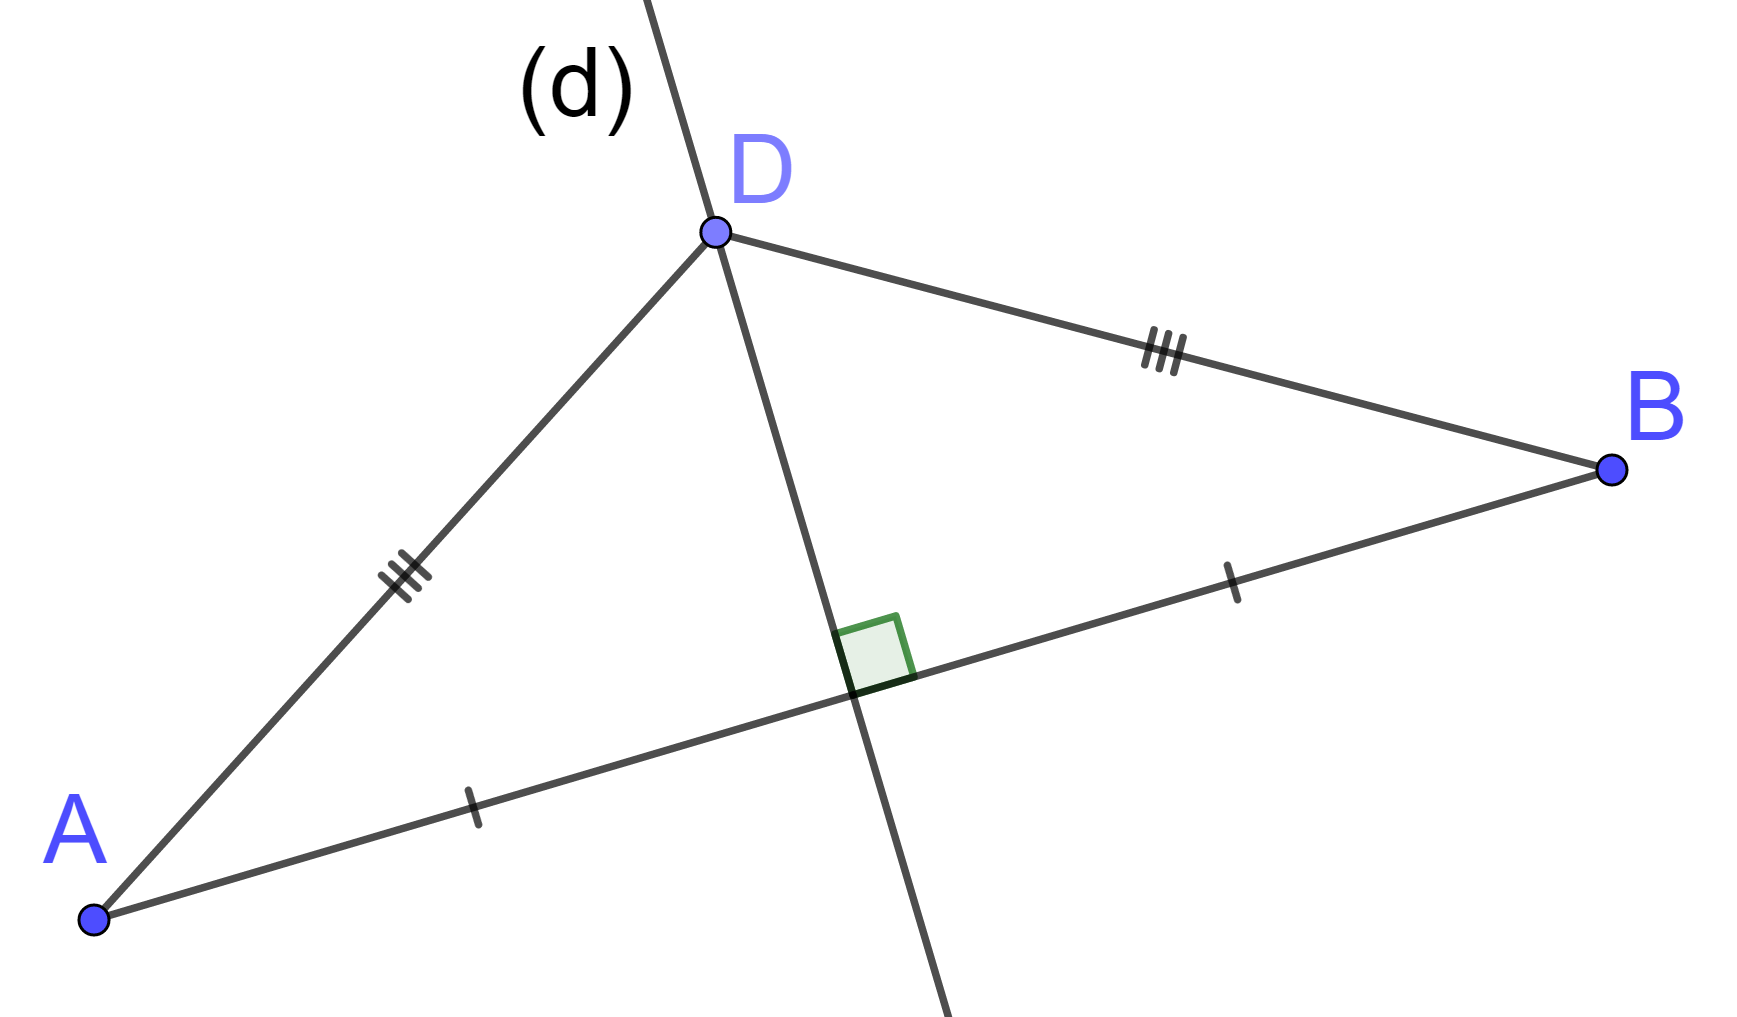
\includegraphics[scale=0.1]{med2}
			\end{center}

			
		\end{enumerate}
	
	
\end{myexs}

\end{frame}

\begin{frame}
	\begin{myprops}
		\begin{itemize}
			\item \textbf{Si} un point appartient à la médiatrice d'un segment, \textbf{alors} ce point est à la même distance des extrémités de ce segment. 
			\item \textbf{Si} un point est à la même distance des extrémités d'un segment, \textbf{alors} il appartient à la médiatrice de ce segment. 			
		\end{itemize}
	\end{myprops}
	
	
	\begin{myexs}
		\begin{enumerate}
						
			\item On a $EG=GF$, $EH=HF$ et $EI=IF$, donc les points $G$, $H$ et $I$ appartiennent tous à la médiatrice du segment $[EF]$.
			
			\begin{center}
				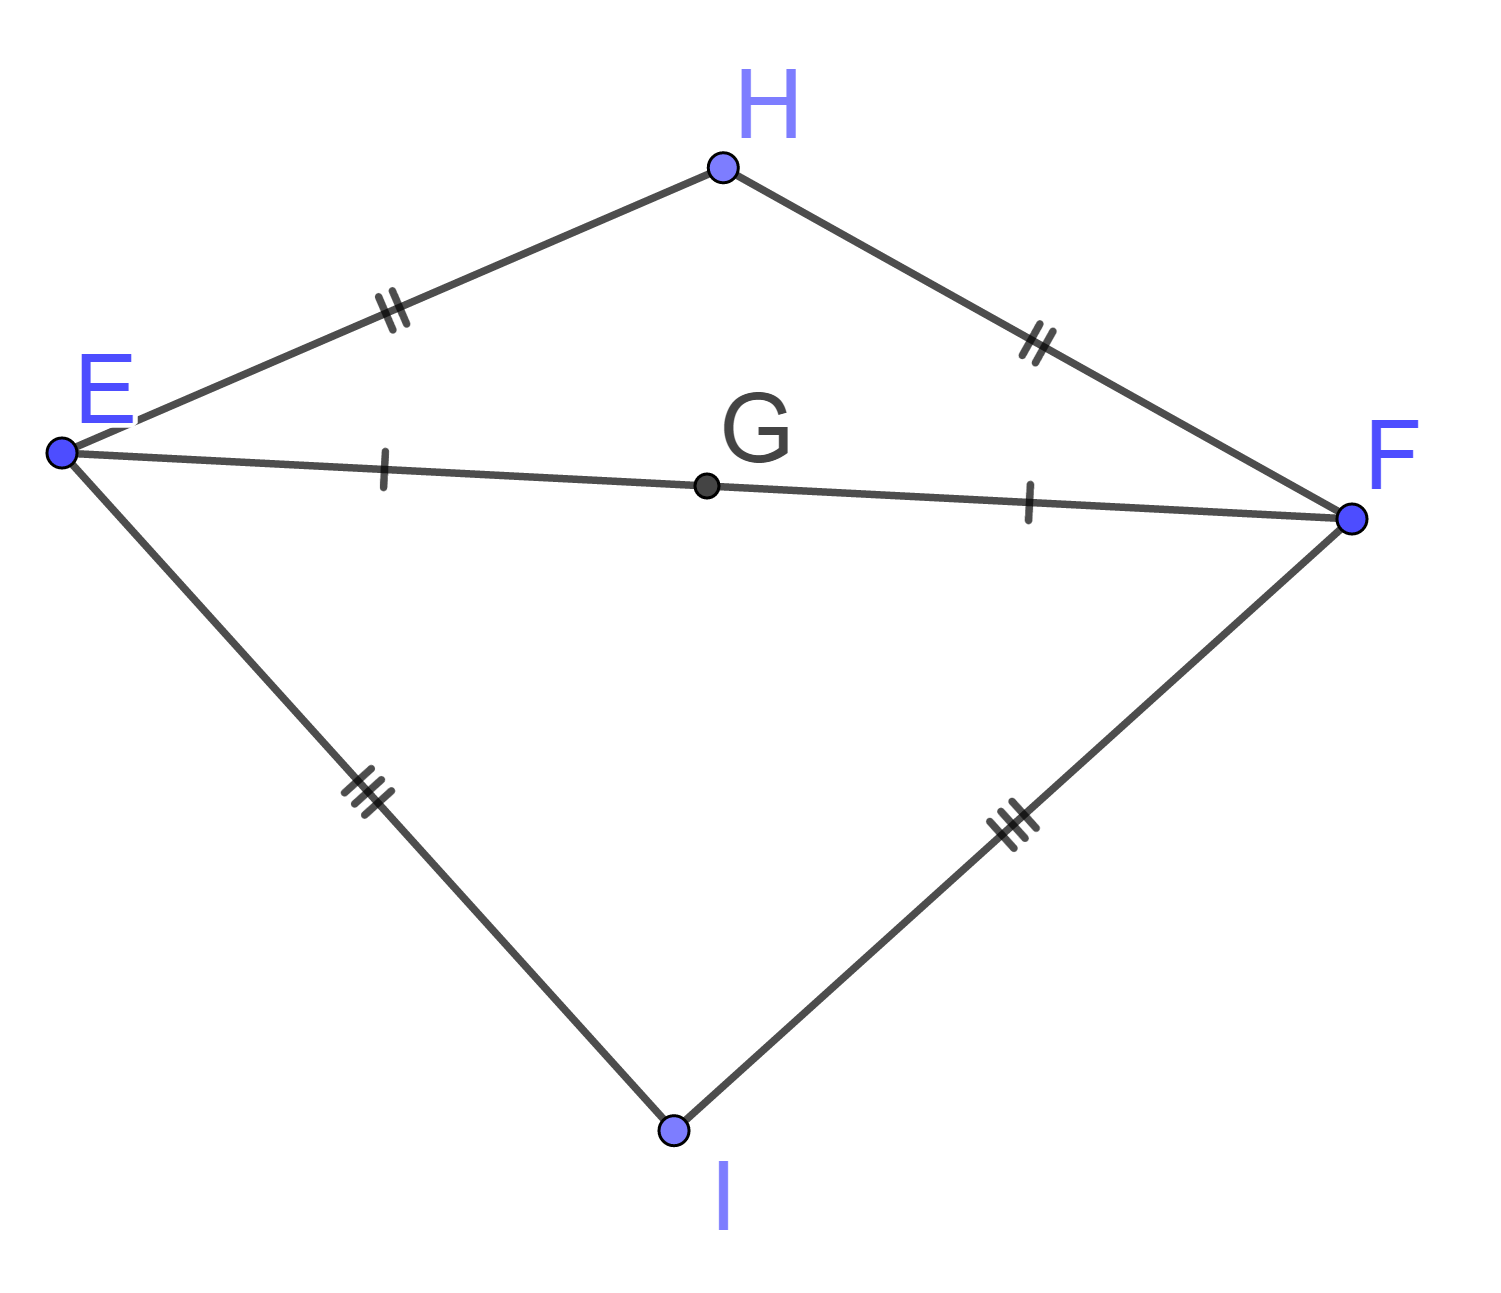
\includegraphics[scale=0.1]{med3}
			\end{center}
			
		\end{enumerate}
		
		
	\end{myexs}
	
\end{frame}

\section{Propriétés de la symétrie}


\begin{frame}
	\begin{myprops}
		\begin{itemize}
				\item Si des points sont alignés, alors leurs symétriques par rapport à une droite sont \kword{aussi alignés}.\pause
				\item Si deux segments sont symétriques par rapport à une droite, alors ils ont la \kword{même longueur}.\pause
				%\item Si deux angles sont symétriques par rapport à une droite, alors ils ont la \kw{même mesure}.
				\item Si deux cercles sont symétriques par rapport à une droite, alors ils ont le \kword{même rayon} et leurs \kword{centres sont symétriques}.\pause
		\end{itemize}
		
	\end{myprops}

	\begin{myexs}
		Le symétrique de la droite $(d_1)$ par rapport à $(d)$ est la droite $(d_2)$.
	

		\begin{center}
			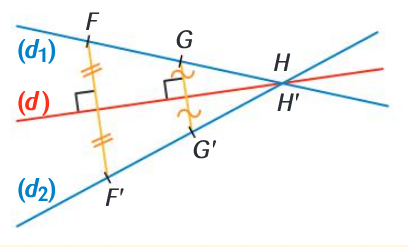
\includegraphics[scale=0.4]{prop1}
		\end{center}
	\end{myexs}
\end{frame}

\begin{frame}
	\begin{myprops}
		\begin{itemize}
			\item Si des points sont alignés, alors leurs symétriques par rapport à une droite sont \kword{aussi alignés}.
			\item Si deux segments sont symétriques par rapport à une droite, alors ils ont la \kword{même longueur}.
			%\item Si deux angles sont symétriques par rapport à une droite, alors ils ont la \kw{même mesure}.
			\item Si deux cercles sont symétriques par rapport à une droite, alors ils ont le \kword{même rayon} et leurs \kword{centres sont symétriques}.
		\end{itemize}
		
	\end{myprops}
	
	\begin{myexs}
		$[IJ]$ et $[I'J']$ sont symétriques par rapport à la droite $(d)$, donc $IJ = I'J'$.
	
		\begin{center}
			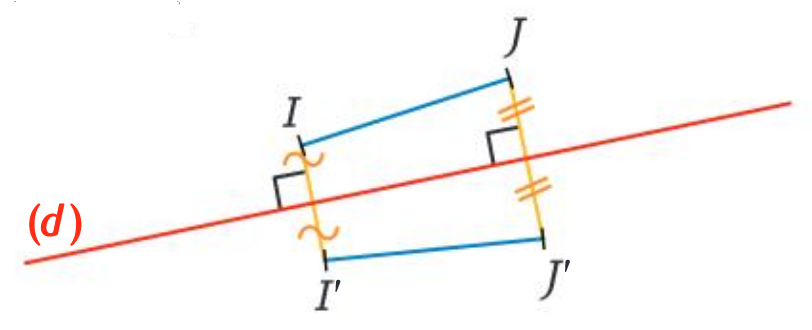
\includegraphics[scale=0.3]{prop2}
		\end{center}
	\end{myexs}
\end{frame}


\begin{frame}
	\begin{myprops}
		\begin{itemize}
			\item Si des points sont alignés, alors leurs symétriques par rapport à une droite sont \kword{aussi alignés}.
			\item Si deux segments sont symétriques par rapport à une droite, alors ils ont la \kword{même longueur}.
			%\item Si deux angles sont symétriques par rapport à une droite, alors ils ont la \kw{même mesure}.
			\item Si deux cercles sont symétriques par rapport à une droite, alors ils ont le \kword{même rayon} et leurs \kword{centres sont symétriques}.
		\end{itemize}
		
	\end{myprops}
	
	\begin{myexs}
		Le symétrique du cercle de centre $O$ et de rayon $r$ est le cercle de centre $O'$ et de rayon $r$.
		
		\begin{center}
			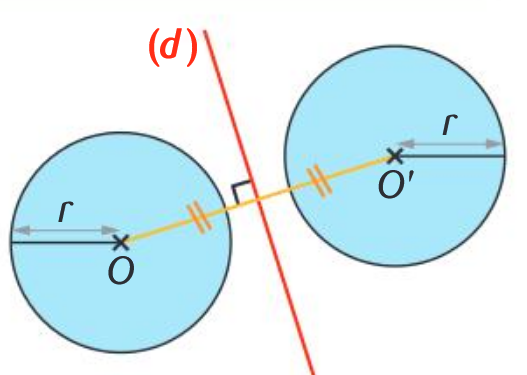
\includegraphics[scale=0.25]{prop3}
		\end{center}
	\end{myexs}
\end{frame}
\end{document}